\subsection{Time of Flight}

Bei \acrshort{tof} handelt es sich um \dots

\pagebreak

\subsection{Photostrom}

Zur Berechnung des theoretisch zu erwartenden Photostrom wird von einer Distanz zur Wand von $10~m$ ausgegangen.

Der Laserstrahl gehe idealisiert mit $0\degree$ zur Wand und werde dort uniform Halbkugel-förmig gestreut. In der
Realität wird der Laser nicht mit $0\degree$ zur Wand gehen und die Streuung wird sich nicht uniform verteilen, sondern
in der Mitte stärker konzentriert sein.

Die Berechnung der empfangenen Strahlungsleistung, der Strahlungsintensität, dem Raumwinkel und dem Photostrom sind in
Formel~\ref{eq:pin}, \ref{eq:ie}, \ref{eq:omega} bzw. \ref{eq:iph} gezeigt.

\begin{equation}\label{eq:pin}
    P_{in} = E_e \cdot A = \frac{I_e}{r^2} \cdot A
\end{equation}
\myequations{Eintreffende Lichtleistung}

\begin{equation}\label{eq:ie}
    I_e = \frac{P_{out}}{\Omega}
\end{equation}
\myequations{Strahlungsintensität}

\begin{equation}\label{eq:omega}
    \Omega = \frac{4\cdot \pi \cdot 0.5}{d}
\end{equation}
\myequations{Raumwinkel}

\begin{equation}\label{eq:iph}
    I_{ph} = S \cdot P_{in}
\end{equation}
\myequations{Photostrom}

\subsubsection{Berechnung mit RLD94PZJ5 und BPV23NF}

Ersten Berechnungen wurden mit der Laserdiode RLD94PZJ5 \cite{rohm2020rld94pzj5_datasheet} und der Photodiode BPV23NF
\cite{vishay2024bpv23nf_datasheet} durchgeführt.

Die relevanten Werte aus den Datenblättern sind in Formel~\ref{eq:rld94pzj5_num} und \ref{eq:rbpv23nf_num} aufgelistet.

\begin{equation}\label{eq:rld94pzj5_num}
    P_{out} = 285~mW
\end{equation}
\myequations{Werte des RLD94PZJ5}

\begin{equation}\label{eq:rbpv23nf_num}
    \begin{split}
        A &= 4.4~mm^2\\
        S &= 0.6~\frac{A}{W}
    \end{split}
\end{equation}
\myequations{Werte des BPV23NF}

Diese Werte eingesetzt in Formel~\ref{eq:ie}, \ref{eq:pin} und \ref{eq:iph} ergibt die Resultate in
Formel~\ref{eq:rld94pzj5_rbpv23nf_num}.

\begin{equation}\label{eq:rld94pzj5_rbpv23nf_num}
    \begin{split}
        I_e    &= \frac{P_{out}}{\Omega} = \frac{285~mW}{\frac{4\cdot \pi \cdot 0.5}{d}} = \frac{285~mW}{\frac{4\cdot \pi \cdot 0.5}{10~m}} = 45~\frac{mW}{sr}\\
        P_{in} &= \frac{I_e}{r^2} \cdot A = 45~\frac{mW}{sr} \cdot 4.4~mm^2 = 2~nW\\
        I_{ph} &= S \cdot P_{in} = 0.6~\frac{A}{W} \cdot 2~nW = 1.2~nA
    \end{split}
\end{equation}
\myequations{Nummerische Resultate mit RLD94PZJ5 und BPV23NF}

\subsubsection{Berechnung mit RLD65NZX1 and NJL6401R-3}

Die Laserdiode RLD94PZJ5 hat im Bezug auf diese Projektarbeit zwei Nachteile: Sehr hohe Leistung, welche für das
menschliche Auge gefährlich werden kann und ein Wellenlängenbereich, der für das menschliche Auge nicht sichtbar ist.

Aus diesen Gründen wurde eine zweite Laserdiode evaluiert: RLD65NZX1 \cite{rohm2019rld65nzx1_datasheet}. Gepaart wird
sie mit der Photodiode NJL6401R-3 \cite{jrc2014njl6401r3_datasheet}. Die folgenden Berechnungen wurden basierend auf
diesen beiden Komponenten durchgeführt.

Die relevanten Werte aus den Datenblättern sind in Formel~\ref{eq:rld65nzx1_num} und \ref{eq:njl6401r3_num} aufgelistet.

\begin{equation}\label{eq:rld65nzx1_num}
    P_{out} = 10~mW
\end{equation}
\myequations{Werte des RLD65NZX1}

\begin{equation}\label{eq:njl6401r3_num}
    \begin{split}
        A &= 0.7~mm \cdot 0.7~mm = 0.49~mm^2\\
        S &= 0.42~\frac{A}{W}
    \end{split}
\end{equation}
\myequations{Werte des NJL6401R-3}

Diese Werte eingesetzt in Formel~\ref{eq:ie}, \ref{eq:pin} und \ref{eq:iph} ergibt die Resultate in
Formel~\ref{eq:rld65nzx1_njl6401r3_num}.

\begin{equation}\label{eq:rld65nzx1_njl6401r3_num}
    \begin{split}
        I_e    &= \frac{P_{out}}{\Omega} = \frac{10~mW}{\frac{4\cdot \pi \cdot 0.5}{d}} = \frac{10~mW}{\frac{4\cdot \pi \cdot 0.5}{10~m}} = 1.6~\frac{mW}{sr}\\
        P_{in} &= \frac{I_e}{r^2} \cdot A = 45~\frac{mW}{sr} \cdot 0.49~mm^2 = 8~pW\\
        I_{ph} &= S \cdot P_{in} = 0.42~\frac{A}{W} \cdot 8~pW = 3.3~pA
    \end{split}
\end{equation}
\myequations{Nummerische Resultate mit RLD65NZX1 and NJL6401R-3}

\subsubsection{Berechnung mit Empfangs-Linse}

Auf Vorschlag der Dozenten wurden verschiedene Optiken aus einem Baukasten-System von QIOPTIQ ausprobiert.
Besonders vielversprechend erschien hierbei eine Linse mit einem Durchmesser von 17~mm bei einer Brennweite von
40~mm. Die Linse ist in Abbildung~\ref{fig:lens} dargestellt.

\begin{figure}[H]
    \centering
    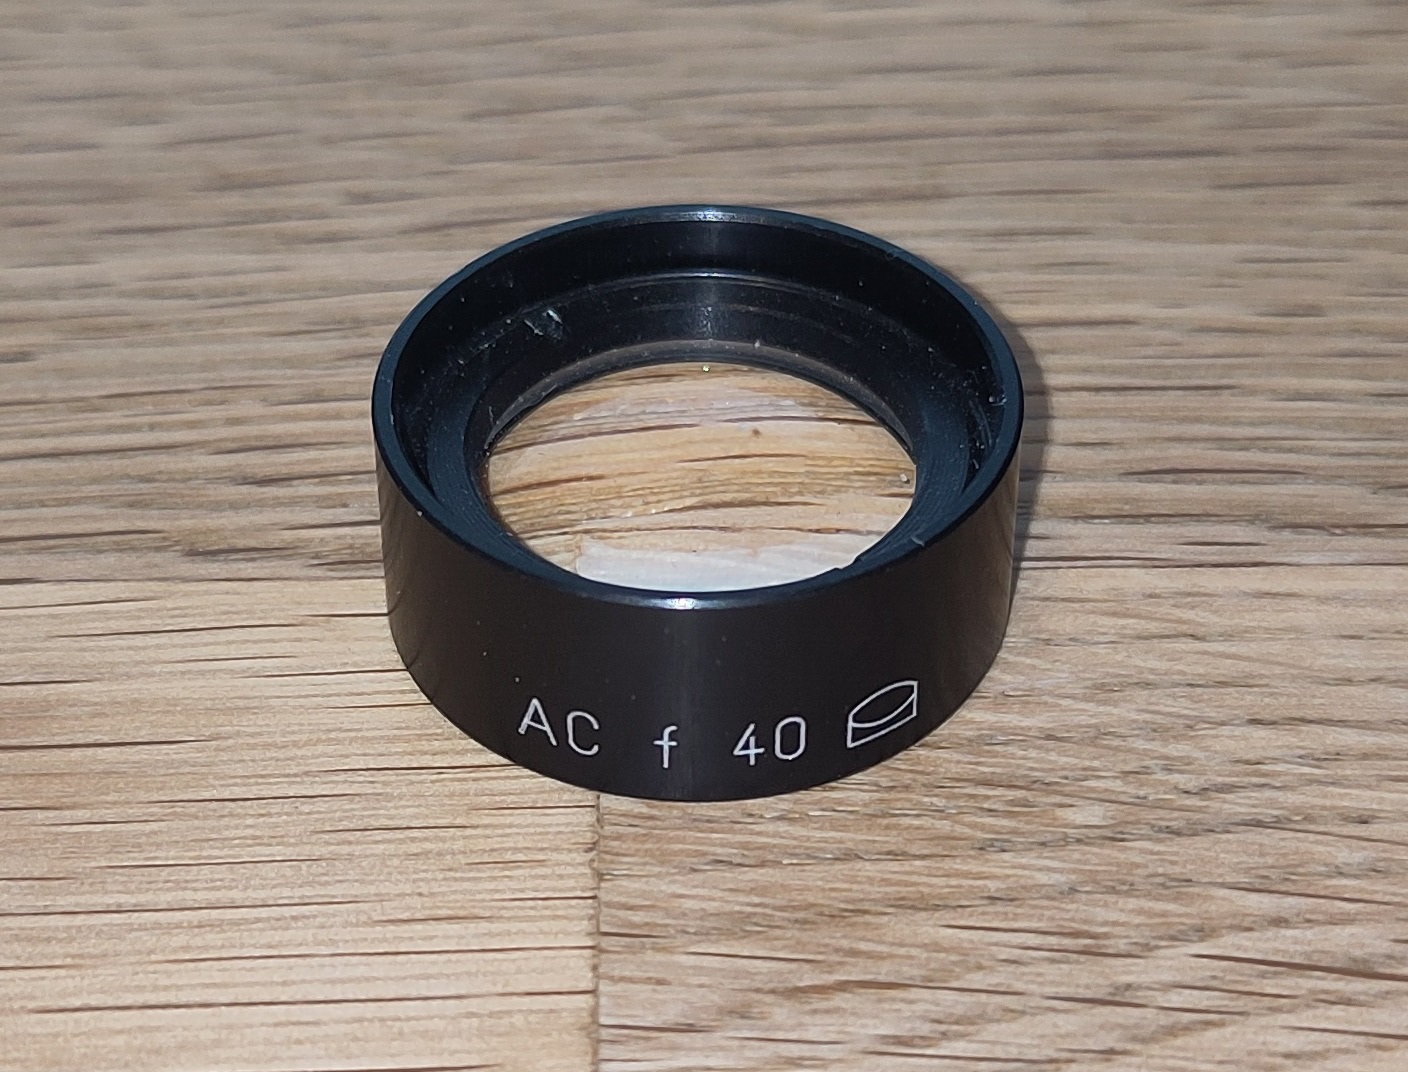
\includegraphics[width=0.5\textwidth]{graphics/photo_lens.jpg}
    \caption{Linse von QIOPTIQ}\label{fig:lens}
\end{figure}

Eine Solche Linse vergrössert die effektive Fläche, auf welcher der Lichtstrom empfangen werden kann, was
eine höhere Empfangsleistung, sprich einen höheren Lichtstrom zur Folge hat.

Im Idealfall kann diese Optik die Fläche um etwa folgenden Faktor vergrössern:

\begin{equation}\label{eq:njl6401r3_lens}
    A' = \frac{A_{L}}{A_{PD}} = \frac{(\frac{17~mm}{2})^2 \cdot \pi}{0.49~mm^2} = 463.2
\end{equation}
\myequations{Vergrösserung der Empfangsfläche durch Linse}

\textcolor{red}{TODO: Wollen wir hier noch eine bessere Annäherung für den Laser machen?}

\pagebreak

\subsection{Transimpedanzverstärker}

Bei einem \acrfull{tia} handelt es sich um \dots
